\documentclass[border=3pt]{standalone}
\usepackage{graphicx}
% source lives in fig/src/; thumbnails live in fig/ -> search both bases so the
% figure compiles whether tectonic resolves relative to the source or the CWD.
\graphicspath{{../}{fig/}{./}}
\usepackage{fontawesome5}   % professional vector icons (embed as crisp glyphs)
\usepackage{tikz}
\usetikzlibrary{arrows.meta,positioning,backgrounds,fit,shapes.geometric,calc,shadows.blur}
\definecolor{wacvblue}{rgb}{0.19,0.47,0.73}
\definecolor{amber}{rgb}{0.90,0.56,0.09}
\definecolor{evalgreen}{rgb}{0.14,0.56,0.44}
\definecolor{slate}{rgb}{0.28,0.33,0.41}
% small inline glyphs for the lane pills (drawn, so no font dependency)
\newcommand{\playicon}{\raisebox{-0.1ex}{\tikz[baseline]{\fill[white] (0,-0.5mm)--(0,1.5mm)--(1.6mm,0.5mm)--cycle;}}}
\newcommand{\pulseicon}{\raisebox{0.1ex}{\tikz[baseline]{\draw[white,line width=0.45pt,line cap=round,line join=round]
   (0,0.3mm)--(0.6mm,0.3mm)--(1.1mm,1.5mm)--(1.7mm,-0.9mm)--(2.3mm,0.5mm)--(2.9mm,0.5mm);}}}
% professional stage icon inside a chip (Font Awesome glyph, colour-matched)
\newcommand{\stgicon}[2]{{\fontsize{12pt}{12pt}\selectfont\textcolor{#1}{#2}}}
\begin{document}
  \begin{tikzpicture}[
    font=\small,
    softshadow/.style={blur shadow={shadow blur steps=7, shadow xshift=0pt,
                       shadow yshift=-0.8pt, shadow opacity=30, shadow blur radius=1.3pt}},
    base/.style={draw, line width=0.8pt, rounded corners=4pt, align=center,
                 minimum height=10mm, text width=25mm, inner sep=5pt, softshadow},
    src/.style={base, shade, top color=slate!2, bottom color=slate!16, draw=slate!55},
    vid/.style={base, shade, top color=wacvblue!5, bottom color=wacvblue!30, draw=wacvblue!70},
    eeg/.style={base, shade, top color=amber!7,  bottom color=amber!32,  draw=amber!80},
    task/.style={base, text width=20mm, shade, top color=slate!2, bottom color=slate!13, draw=slate!50},
    ev/.style={base, text width=27mm, shade, top color=evalgreen!5, bottom color=evalgreen!30,
               draw=evalgreen!70},
    vimg/.style={draw, line width=0.8pt, draw=wacvblue!60, fill=white,
                 rounded corners=3pt, align=center, inner sep=2pt, text width=32mm, softshadow},
    eimg/.style={draw, line width=0.8pt, draw=amber!75, fill=white,
                 rounded corners=3pt, align=center, inner sep=2pt, text width=32mm, softshadow},
    varr/.style={-{Stealth[round,length=2.6mm,width=2.4mm]}, line width=1.2pt, draw=wacvblue!75},
    earr/.style={-{Stealth[round,length=2.6mm,width=2.4mm]}, line width=1.2pt, draw=amber!85!black},
    narr/.style={-{Stealth[round,length=2.6mm,width=2.4mm]}, line width=1.2pt, draw=slate!65},
    hnum/.style={circle, shade, top color=wacvblue!95, bottom color=wacvblue!62, text=white,
                 font=\scriptsize\bfseries, inner sep=0.5pt, minimum size=5mm,
                 draw=wacvblue!80, line width=0.4pt, softshadow},
    htxt/.style={anchor=center, align=center, font=\footnotesize, text=slate,
                 text width=22mm, inner sep=1pt},
    pill/.style={rounded corners=2.5pt, inner sep=3pt, font=\bfseries\scriptsize,
                 text=white, softshadow},
    iconchip/.style={rounded corners=1.6pt, minimum size=7mm, inner sep=0pt,
                     fill=slate!7, draw=slate!35, line width=0.4pt, softshadow},
  ]
  % --- main-flow nodes (lanes at y=+/-1.4, compact)
  \node[src]  (raw)  at (0,0)       {Synchronized\\video--EEG};
  \node[src]  (clip) at (3.4,0)     {Clip extraction:\\seizure $+$ matched\\non-seizure};
  \node[vimg] (vf)   at (7.3,1.35)  {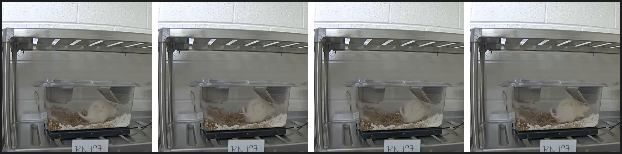
\includegraphics[width=30mm]{filmstrip.png}\\[1pt]
                                     {\scriptsize\itshape sampled frames, 16--32\,@\,$224^2$}};
  \node[vid]  (vm)   at (11.1,1.35) {Video backbone\\{\scriptsize R(2+1)D\,\dots\,MViTv2}\\{\scriptsize 10 compared}};
  \node[eimg] (ew)   at (7.3,-1.35) {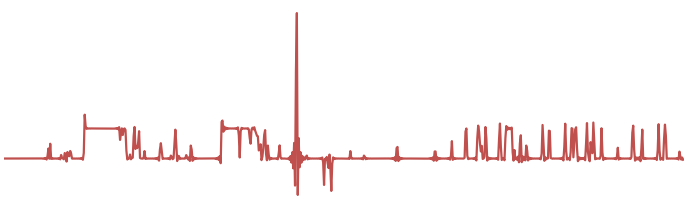
\includegraphics[width=30mm]{eeg_clip.png}\\[1pt]
                                     {\scriptsize\itshape EEG window, 6\,s\,@\,125\,Hz}};
  \node[eeg]  (em)   at (11.1,-1.35){EEG backbone\\GRU$\,\dots\,$XGBoost\\{\scriptsize 7 compared, pooled to clip}};
  \node[task] (tkv)  at (14.4,1.35) {Task head\\2 / 3 / 5-class};
  \node[task] (tke)  at (14.4,-1.35){Task head\\2 / 3 / 5-class};
  \node[ev]   (ev)   at (17.6,0)    {Session-disjoint\\eval: macro-F1,\\AUROC, per-subj.};
  % --- swimlane bands + pills (behind the nodes)
  \begin{scope}[on background layer]
    \shade[top color=wacvblue!13, bottom color=wacvblue!3, draw=wacvblue!30, line width=0.5pt,
           rounded corners=9pt] ($(vf.north west)+(-4mm,4mm)$) rectangle ($(tkv.south east)+(4mm,-4mm)$);
    \shade[top color=amber!4, bottom color=amber!13, draw=amber!35, line width=0.5pt,
           rounded corners=9pt] ($(ew.north west)+(-4mm,4mm)$) rectangle ($(tke.south east)+(4mm,-4mm)$);
  \end{scope}
  \node[pill, shade, top color=wacvblue!88, bottom color=wacvblue!58, anchor=south west]
        at ($(vf.north west)+(-4mm,1.2mm)$) {\playicon~VIDEO};
  \node[pill, shade, top color=amber!80!black, bottom color=amber!55!black, anchor=north west]
        at ($(ew.south west)+(-4mm,-1.2mm)$) {\pulseicon~EEG};
  % --- stage headers: pro icon chip + numbered badge + label (icon left of badge)
  \node[htxt] (h1) at (0,3.05)    {Synchronized\\recording};
  \node[hnum] (n1) at ([xshift=-0.6mm]h1.west) {1};
  \node[iconchip, anchor=east] (i1) at ([xshift=-1.3mm]n1.west) {\stgicon{slate}{\faVideo}};
  \node[htxt] (h2) at (3.4,3.05)  {Clip\\extraction};
  \node[hnum] (n2) at ([xshift=-0.6mm]h2.west) {2};
  \node[iconchip, anchor=east] (i2) at ([xshift=-1.3mm]n2.west) {\stgicon{slate}{\faCut}};
  \node[htxt] (h3) at (9.2,3.05)  {Per-modality\\encoders};
  \node[hnum] (n3) at ([xshift=-0.6mm]h3.west) {3};
  \node[iconchip, anchor=east] (i3) at ([xshift=-1.3mm]n3.west) {\stgicon{slate}{\faProjectDiagram}};
  \node[htxt] (h4) at (14.4,3.05) {Task\\head};
  \node[hnum] (n4) at ([xshift=-0.6mm]h4.west) {4};
  \node[iconchip, anchor=east] (i4) at ([xshift=-1.3mm]n4.west) {\stgicon{slate}{\faSignal}};
  \node[htxt] (h5) at (17.5,3.05) {Session-disjoint\\evaluation};
  \node[hnum] (n5) at ([xshift=-0.6mm]h5.west) {5};
  \node[iconchip, anchor=east] (i5) at ([xshift=-1.3mm]n5.west) {\stgicon{slate}{\faChartLine}};
  % --- main-flow arrows (lane-colored, curved branch + merge)
  \draw[narr] (raw) -- (clip);
  \draw[varr] (clip.east) to[out=28,in=180] (vf.west);
  \draw[earr] (clip.east) to[out=-28,in=180] (ew.west);
  \draw[varr] (vf) -- (vm);
  \draw[earr] (ew) -- (em);
  \draw[varr] (vm) -- (tkv);
  \draw[earr] (em) -- (tke);
  \draw[varr] (tkv.east) to[out=0,in=148] (ev.north west);
  \draw[earr] (tke.east) to[out=0,in=-148] (ev.south west);
\end{tikzpicture}
\end{document}
